\documentclass{article}
\usepackage{amsmath}
\usepackage{tcolorbox}
\usepackage[margin=0.5in]{geometry} 
\usepackage{amsmath,amsthm,amssymb,amsfonts, fancyhdr, color, comment, graphicx, environ}
\usepackage{float}
\usepackage{xcolor}
\usepackage{mdframed}
\usepackage[shortlabels]{enumitem}
\usepackage{indentfirst}
\usepackage{mathrsfs}
\usepackage{hyperref}
\graphicspath{{./}{gr/}}
\makeatletter
\newcommand*{\rom}[1]{\expandafter\@slowromancap\romannumeral #1@}
\makeatother
% Change enumerate labels to (a), (b), (c), ...
% Define a new environment for problems
\newcounter{problemCounter}
\newtcolorbox{problem}[2][]{colback=white, colframe=black, boxrule=0.5mm, arc=4mm, auto outer arc, title={\ifstrempty{#1}{Problem \stepcounter{problemCounter}\theproblemCounter}{#1}}}

% \renewcommand{\labelenumi}{\alph{enumi})}
\def\zz{{\mathbb Z}}
\def\R{{\mathbb R}}
\def\qq{{\mathbb Q}}
\def\cc{{\mathbb C}}
\def\N{{\mathbb N}}
\def\ss{{\mathbb S}}

\newcommand{\p}{\partial}
\renewcommand{\vec}[1]{\mathbf{#1}}
\newcommand{\vx}{\vec{x}}
\newcommand{\Lag}{\mathcal{L}}
\newcommand{\sep}{\,:\,}


\newtheorem{theorem}{Theorem}[section]
\newtheorem{corollary}{Corollary}[theorem]
\newtheorem{lemma}[theorem]{Lemma}
\newtcolorbox{proposition}[1][]{colback=white, colframe=blue, boxrule=0.5mm, arc=4mm, auto outer arc, title={Proposition #1}}
\newtcolorbox{definition}[1][]{colback=white, colframe=violet, boxrule=0.5mm, arc=4mm, auto outer arc, title={Definition #1}}
\newcommand{\Zmod}[1]{\zz/#1\zz}
\newcommand{\partFrac}[2]{\frac{\partial #1}{\partial #2}}

\newcommand\Mydiv[2]{%
$\strut#1$\kern.25em\smash{\raise.3ex\hbox{$\big)$}}$\mkern-8mu
        \overline{\enspace\strut#2}$}

\begin{document}

\begin{center}
    Math 714
    \hfill Homework 2
    \hfill \textit{Stephen Cornelius}
\end{center}

\textbf{Note:} I originally did this homework in a Jupyter Notebook. I will include the notebook for the coding portion of this homework. I could not get the code to render in \LaTeX~so I will just include the answers here and the notebook will have the code, scratchwork, and results.


\begin{problem} \\
    \textbf{Iterative Methods:} \\
    \begin{enumerate}[(a)]
        \item Consider the $2 \times 2$ matrix
                $$
                        A = \begin{pmatrix}
                        1 & p \\
                        -p & 1
                        \end{pmatrix}.
                $$
                Under what conditions will the Jacobi and Gauss-Seidel methods converge?
        \item Consider the $n \times n$ matrix
                $$
                    C = \begin{pmatrix}
                    3 & -1 \\
                    -1 & 3 & -1 \\
                    & -1 & 3 & -1 \\
                    &    & & \ddots &  \\
                    & & & -1 & 3 & -1  \\
                    & & & & -1 & 3 
                    \end{pmatrix}.
                $$
                Starting from $u_0 \in \mathbb{R}^n$, for which values of $\omega \in \mathbb{R}$ does the iteration 
                $$ u_{k+1} = u_k + \omega(b-Cu_k) $$
                for $k = 0,1,2,\dots$ converge to a solution of $Cu = b$? What iterative method from the lectures does this most closely resemble? How is it different?
    \end{enumerate}
\end{problem}

\begin{enumerate}[(a)]
    \item From the text book we have that "both methods can be analyzed by viewing them as based on splitting of the matrix $A$ into $A = M - N$ where $M$ and $N$ are two $m \times m$ matrices. Then the system $Au = f$ can be rewritten as $Mu - Nu = f \implies Mu = Nu + f$, "
    \begin{enumerate}[i.)]
        \item For the Jacobi method we can let $M = D$ and $N = L + U$ where $D$ is the diagonal of $A$, $L$ is the lower triangular portion of $A$, and $U$ is the upper triangular portion of $A$. So then we have that $Du^{k+1} = (L + U)u^k + f$. Then we have that $u^{k+1} = D^{-1}(L + U)u^k + D^{-1}f$. So then the iteration matrix is $T_J = D^{-1}(L + U)$. So we need to find the spectral radius $\rho(T_J)$. We have that
        \begin{align*}
            T_J &= D^{-1}(L + U) \\
            &= \begin{pmatrix}
                1 & 0 \\
                0 & 1
            \end{pmatrix}^{-1} \left( \begin{pmatrix}
                0 & 0 \\
                p & 0
            \end{pmatrix} + \begin{pmatrix}
                0 & p \\
                0 & 0
            \end{pmatrix} \right) \\
            &= \begin{pmatrix}
                1 & 0 \\
                0 & 1
            \end{pmatrix} \begin{pmatrix}
                0 & p \\
                p & 0
            \end{pmatrix} \\
            &= \begin{pmatrix}
                0 & p \\
                p & 0
            \end{pmatrix}.
        \end{align*}
        Calculating the eigenvalues we have $\det(T_J - \lambda I) = \det \begin{pmatrix}
            -\lambda & p \\
            p & -\lambda
        \end{pmatrix} = \lambda^2 - p^2$. So then the eigenvalues are $\lambda = \pm p$. So then we have that $\rho(T_J) = \max\{\vert p \vert, \vert -p \vert\} = \vert p \vert$. So then we need $\rho(T_J) < 1$ for convergence. So then the Jacobi method converges when $\vert p \vert < 1$.
          

        \newpage
        \item For the Gauss-Seidel method we can let $M = D - L$ and $N = U$. So then we have that $(D - L)u^{k+1} = Uu^k + f$. Then we have that $u^{k+1} = (D - L)^{-1}Uu^k + (D - L)^{-1}f$. So then the iteration matrix is $T_{GS} = (D - L)^{-1}U$. So we need to find the spectral radius $\rho(T_{GS})$. We have that
        \begin{align*}
            T_{GS} &= (D - L)^{-1}U \\
            &= \left( \begin{pmatrix}
                1 & 0 \\
                0 & 1
            \end{pmatrix} - \begin{pmatrix}
                0 & 0 \\
                p & 0
            \end{pmatrix} \right)^{-1} \begin{pmatrix}
                0 & p \\
                0 & 0
            \end{pmatrix} \\
            &= \begin{pmatrix}
                1 & 0 \\
                p & 1
            \end{pmatrix} \begin{pmatrix}
                0 & p \\
                0 & 0
            \end{pmatrix} \\
            &= \begin{pmatrix}
                0 & p \\
                0 & p^2
            \end{pmatrix}.
        \end{align*}
        Calculating the eigenvalues we have $\det(T_{GS} - \lambda I) = \det \begin{pmatrix}
            -\lambda & p \\
            0 & p^2 - \lambda
        \end{pmatrix} = -\lambda(p^2 - \lambda)$. So then the eigenvalues are $\lambda = 0$ and $\lambda = p^2$. So then we have that $\rho(T_{GS}) = \max\{0, \vert p^2 \vert\} = p^2$. So then we need $\rho(T_{GS}) < 1$ for convergence. So then the Gauss-Seidel method converges when $|p| < 1$.
    \end{enumerate}
    \item We are tasked with finding the values of $\omega \in \mathbb{R}^n$ such that $u_{k+1} = u_k + \omega(b - Cu_k)$ converges. If we let $T = I - \omega C$ we have 
    $$ u_{k+1} = u_k + \omega (b - Cu_k) = u_k + \omega b - \omega Cu_k = u_k(I - \omega C) + \omega b = Tu_k + \omega b.$$ 
    So then we need that the spectral radius of $T$ needs to be less than $1$. So we find $\rho(T)$. From the article (see bibliography), we have that $$ \rho(T) = \max \left\{ \left\vert (1 - 3\omega) + 2\sqrt{\vert (- \omega)^2 \vert} e^{\frac{i(\alpha + \beta)}{2}} \cos \frac{\pi}{n + 1}\right\vert, \left\vert (1 - 3\omega) + 2\sqrt{\vert (- \omega)^2 \vert} e^{\frac{i(\alpha + \beta)}{2}} \cos \frac{n \pi}{n + 1}\right\vert\right\}$$ where  in this case, 
    $$\alpha = \beta = \arg(-\omega) = \left\{\begin{matrix} 
        \pi & \text{if } \omega > 0 \\ 
        0 & \text{if } \omega < 0 
        \end{matrix}\right. .$$
    In either case we have that $\alpha + \beta \approx 2\pi$. So then $$\rho(T) = \max \left\{ \left\vert (1 - 3\omega) - 2 \omega \cos \frac{\pi}{n + 1}\right\vert, \left\vert (1 - 3\omega) - 2 \omega \cos \frac{n \pi}{n + 1}\right\vert\right\} .$$
    Then we need $\rho(T) < 1$. Then we have that the smallest interval on which $\omega$ converges is when $n = 1$ and then we have that the method converges when $0 < \omega < \frac{2}{3}$. That is, $\left\vert (1 - 3\omega) - 2 \omega \cos \frac{\pi}{2}\right\vert < 1 \iff 0 < \omega < \frac{2}{3}$.

    Based on my observations, I would conclude that the iterative method from class that most closely resembles this method would be gradient descent. The difference would be that gradient descent finds the largest value of the gradient and this method uses more of a fixed parameter rather than optimal step sizes.

    \textit{Comment(s):}
    For help with this problem I used Desmos to graph $\rho(T)$. From observation $\omega$ always converges when $0 < \omega < \frac{2}{3}$ but since $n$ varies we can see that as $n \to \infty$ we have that the interval for $\omega$ becomes $0 < \omega < 2$.
\end{enumerate}



\begin{problem} \\
    \textbf{Triangular domain revisited with conjugate gradient:} \\
    Question 4 of the first homework assignment looked at solving the Poisson equation
   $$ \nabla^2u = f$$
   on the triangular domain $T$ with vertices $(0,0), (1,0),$ and $(s,\frac{1}{2})$ where $s = \frac{\sqrt{3}}{2}$. Dirchlet boundary conditions $u = 0$ are applied on the boundary $\partial T$. For $n \in \mathbb{N}$ and $h = \frac{1}{n}$, the domain is descretized with points 
   $$ \vec{x}_{i,j} = (h(i + \frac{1}{2}j), hsj) $$
   for $0 \leq i \leq n, 0 \leq j \leq n-i$. The points where $i = 0, j = 0,$ of $i + j = n$ are boundary points, and all others are interior. Let $u_{i,j}$ be the numberical approximation for $u(x_{i,j})$. The Laplacian is discretized with points
   $$ \nabla^2_6u_{i,j} = \frac{2(-6 u_{i,j} + u_{i+1,j} + u_{i,j-1} + u_{i-1,j+1} +u_{i-1,j} + u_{i,j+1} + u_{i+1,j-1})}{3h^2}. $$
   As in Homework 1, consider solving the equation $\nabla^2u = f$ using the $f$ that creates the exact solution
   $$ u^{\text{ex}}(x,y) = \left( (2y-\sqrt{3})^2- 3(2x-1)^2 \right) \sin y. $$
   The problem can be expressed as a linear system $Au = f$ where $u \in \mathbb{R}^N$ is the solution vector at the $N = (n-1)(n-2)/2$ interior grid points. Define an approximate $2$-norm as 
   $$ ||r||_2 = \sqrt{\frac{s}{2n^2} \sum_{j=1}^{n-1} \sum_{i=1}^{n-j-1} r_{i,j}^2} $$
   for a vector $r$ describing a field on the grid.

   \begin{enumerate}[(a)]
    \item For a range of grid sizes from $n=10$ up to at least $n=160$ measure the wall-clock time $T_n$ to solve the system using your code. By making a log--log plot of $T_n$ versus $n$, fit the timing data to $$T_n = a n^b,$$ and comment on the exponent $b$.
    \item Write a code to implement the conjugate gradient (CG) algorithm to solve $Au=f$. Your code should not explicitly build $A$ as a dense matrix. It should either represent $A$ as a sparse matrix, or contain a function that can directly compute $Aq$ for a given vector $q$. The CG algorithm should terminate when $||r||_2 < 10^{-10}$, where $r$ is the residual vector. For the case when $n=40$ test that your program gives the same results as the original version.
    \item For $n=10,20,40,80,160$, calculate the number of iterations $k$ required in order to reach the termination criterion.
    \item Measure the wall-clock time of the CG algorithm to solve the linear system for a range of grid sizes from $n=10$ up to at least $n=160$. Fit the data to $T_n = an^b$ and comment on how the exponent compares to your result from part (a).
    \item Consider the block Jacobi preconditioner $M$ with block sizes of $w=\lfloor \sqrt{N} \rfloor$. In general, $w$ will not evenly divide $N$, and therefore let the final block of $M$ be smaller. Implement the preconditioned CG algorithm, and repeat part (c) to measure the number of iterations required to reach the termination criterion.
    \item Repeat part (d), fitting the timing data to $T_n = an^b$
   \end{enumerate}
\end{problem}

\newpage
\begin{enumerate}[(a)]
    \item Please see \texttt{Homework2.ipynb} for the code and results. From the image below we have that the exponent $b \approx 3.606$. This is a bit higher than I expected. I would have guessed that $b$ would be closer to $3$ since the algorithm is $\mathcal{O}(N^2)$ and $N = \frac{(n-1)(n-2)}{2} \approx \frac{n^2}{2}$. So then we would have that the algorithm is $\mathcal{O}(n^4)$. However, I think the extra time could be due to overhead from Python or some other factor.
    \begin{figure}[H]
        \centering
        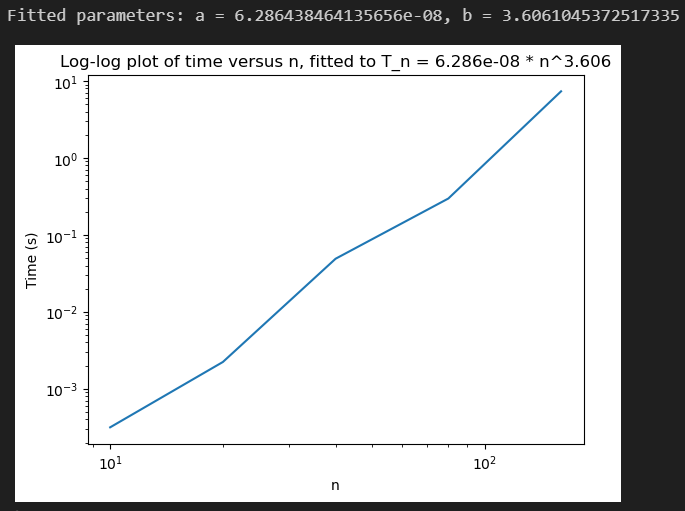
\includegraphics[width=0.4\textwidth]{Q1a.png}
        \caption{Log-Log plot of $T_n$ vs $n$}
        %\label{fig:my_label}
    \end{figure}
    \item Please see \texttt{Homework2.ipynb} for the code and results. \\
    \textbf{Comment:} When my code is ran, for $n = 40$ the norm between my CG algorithm and the poisson\_tri function is consistently $ \approx 5.75936$ but when using np.linalg.solve to solve, the norm between my CG algorithm and np.linalg.solve is consistently $ \approx 4.0477e-14$. 
    \item Below is an image of the table of the number of iterations $k$ required to reach the termination criterion for various values of $n$.
    \begin{figure}[H]
        \centering
        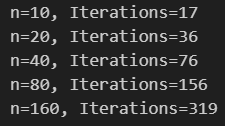
\includegraphics[width=0.4\textwidth]{Q1c.png}
        \caption{Table of number of iterations $k$ vs $n$}
        %\label{fig:my_label}
    \end{figure}
    \item Below is an image of the results for $a$ and $b$ when fitting the data to $T_n = an^b$. From the image we have that $b \approx 3.055$. This is much closer to what I expected. I would have guessed that $b$ would be close to $3$ since the algorithm is $\mathcal{O}(N^2)$ and $N = \frac{(n-1)(n-2)}{2} \approx \frac{n^2}{2}$. So then we would have that the algorithm is $\mathcal{O}(n^4)$. The reason this is lower than part (a) is because the CG algorithm is more efficient than the original algorithm used in part (a).
    \begin{figure}[H]
        \centering
        
\includegraphics[width=0.4\textwidth]{Q1d.png}
        \caption{Results for $a$ and $b$ when fitting the data to $T_n = an^b$}
        %\label{fig:my_label}
    \end{figure}
    \item Below is an image of the table of the number of iterations $k$ required to reach the termination criterion for various values of $n$ when using the block Jacobi preconditioner with block sizes of $w=\lfloor \sqrt{N} \rfloor$.
    \begin{figure}[H]
        \centering
        
\includegraphics[width=0.4\textwidth]{Q2e.png}
        \caption{Table of number of iterations $k$ vs $n$ when using the block Jacobi preconditioner}
        %\label{fig:my_label}
    \end{figure}
    \item Below is an image of the results for $a$ and $b$ when fitting the data to $T_n = an^b$ with the block Jacobi preconditioner.
    \begin{figure}[H]
        \centering
        
\includegraphics[width=0.4\textwidth]{Q2f.png}
        \caption{Results for $a$ and $b$ when fitting the data to $T_n = an^b$ with the block Jacobi preconditioner}
        %\label{fig:my_label}
    \end{figure}
\end{enumerate}







\newpage

\begin{problem} \\ 
    \textbf{ODE Integration Methods:} \\
    \begin{enumerate}[(a)]
        \item Consider solving the differential equation $y' = f(t,y)$ at timepoints $t_k$ with corresponding numerical solutions $y_k$. The multi-step Nystr\"om numerical method is based upon the integral relation 
        $$y(t_{k+1}) = y(t_{k-1}) + \int_{t_{k-1}}^{t_{k+1}} f(t,y) dt.$$ 
        Derive an implicit multi-step numerical method by approximating the integrand $f(t,y)$ with the polynomial interpolant using the function values at $t_{k-2}$, $t_{k-1}$, $t_k$, and $t_{k+1}$. Your method should have the form 
        \[y_{k+1} = y_{k-1} + h(\alpha f_{k-2}+\beta f_{k-1} + \gamma f_k+\eta f_{k+1}) \quad \quad \quad \text{(1)}\]
         where $\alpha$, $\beta$, $\gamma$, and $\eta$ are constants to be determined, $h$ is the timestep interval size, and $f_l=f(t_l,y_l)$ for an arbitrary $l$.
        
        \item Find the exact solution to the second-order differential equation 
        \[ y''(t)+2y'(t) + 26y(t)=0, \quad \quad \quad \text{(2)}\]
        subject to the initial conditions $y(0)=1$, $y'(0)=0$.
        
        \item Write $y''(t)+2y'(t) + 26y(t)=0$ as a coupled system of two first-order differential equations for $\vec{y} = (y,v) = (y,y')$. Solve the system over the interval $0 \leq t \leq 3$ with a timestep of $h = 0.02$ using your multi=step method from part (a).

        Before (1) can be applied, $\vec{y}_1$ and $\vec{y}_2$ must be calculated accurately. Use one of the following two approaches:
        \begin{enumerate}[i.)]
            \item set them based on the exact solution from part (b).
            \item calculate them using the classical fourth-order Runge-Kutta method.
        \end{enumerate}
        Plot the exact and numerical solutions over the range $0 \leq t \leq 3$.

        Make a log-log plot of the absolute error between the numerical and exact values of $y$ at $t = 3$ as a function of $h$, over the range from $h = 10^{-3}$ to $h = 10^{-1}$.

        Show that your method is fourth-order accurate.
        
        \item Suppose that instead of setting $\vec{y}_1$ and $\vec{y}_2$ accurately, you instead make use of forward Euler steps. Create a log-log plot of the absolute error of $y$ at $t=3$ as a function of $h$. Determine the order of accuracy, and discuss why this is the case.
    \end{enumerate}
\end{problem}


\begin{enumerate}[(a)]
    \item % From the text book: The explicit Nystrom methods have the form $U^{n + r} = U^{n + r - 2} + k \sum_{j = 0}^{r=1} \beta_j f(U^{n + j})$ with the $\beta_j$ chosen to give order $r$. The midpoint method is a two-step explicit Nystrom method. A two step Nystrom method is Simpson's rule, $U^{n + 2} = U^n + \frac{2k}{6}(f(U^n) + 4f(U^{n + 1}) + f(U^{n + 2}))$. This reduces to Simpson's rule for quadrature if applied to the ODE $u'(t) = f(t)$.
    First we build the method by replacing $f(t,y)$ on $[t_{k-1},t_{k+1}]$ with the cubic Lagrange interpolant through the four values
    \[
    f_{k-2}=f(t_{k-2},y_{k-2}),; f_{k-1},; f_k,; f_{k+1}.
    \]
    Let $s = \frac{t-t_k}{h}$ be the normalized time variable on the interval $[t_{k-1},t_{k+1}]$,
    so the four interpolation nodes become $s=-2,-1,0,1$ which correspond to $t_{k-2},t_{k-1},t_k,t_{k+1}$. Then we have that the integral in the Nyström relation becomes
   \[
    \int_{t_{k-1}}^{t_{k+1}} f(t,y),dt
    = h\int_{-1}^{1} p(s),ds,
   \]
    where $p(s)$ is the cubic Lagrange interpolant
   \[
    p(s)=f_{k-2}L_{-2}(s)+f_{k-1}L_{-1}(s)+f_k L_0(s)+f_{k+1}L_{1}(s),
   \]
    and $L_j(s)$ are the Lagrange basis polynomials for nodes $-2,-1,0,1$. Then we have that the four basis polynomials are
   \[
    \begin{aligned}
    L_{-2}(s)&=\frac{(s+1)s(s-1)}{(-2+1)(-2-0)(-2-1)}
    =\frac{s(1-s^2)}{6}, \\
    L_{-1}(s)&=\frac{(s+2)s(s-1)}{(-1+2)(-1-0)(-1-1)}
    =\frac{s(s-1)(s+2)}{2}, \\
    L_{0}(s)&=\frac{(s+2)(s+1)(s-1)}{(0+2)(0+1)(0-1)}
    =-\frac{(s-1)(s+1)(s+2)}{2}, \\
    L_{1}(s)&=\frac{(s+2)(s+1)s}{(1+2)(1+1)(1-0)}
    =\frac{s(s+1)(s+2)}{6}.
    \end{aligned}
   \]

    Next, we integrate each basis polynomial over the interval $s \in [-1, 1]$. Starting with $L_{-2}(s)$, which is an odd function, its integral over the symmetric interval is zero, $\int_{-1}^{1} L_{-2}(s),ds=0.$
    Computing the remaining integrals we have,
   \[
    \int_{-1}^{1} L_{-1}(s),ds=\frac{1}{3},\qquad
    \int_{-1}^{1} L_{0}(s),ds=\frac{4}{3},\qquad
    \int_{-1}^{1} L_{1}(s),ds=\frac{1}{3}.
   \]
    Therefore
   \[
    \int_{t_{k-1}}^{t_{k+1}} f(t,y),dt
    = h\Big(0\cdot f_{k-2}+\tfrac{1}{3}f_{k-1}+\tfrac{4}{3}f_k+\tfrac{1}{3}f_{k+1}\Big).
   \]

    Substituting into $y(t_{k+1})=y(t_{k-1})+\int_{t_{k-1}}^{t_{k+1}} f(t,y),dt$ and replacing the exact solution values by the numerical approximations ($y_{k\pm j}$) yields the implicit multi-step Nyström method with
   \[
    \alpha=0,\qquad \beta=\tfrac{1}{3},\qquad \gamma=\tfrac{4}{3},\qquad \eta=\tfrac{1}{3}.
   \]

    So the scheme is
   \[
    y_{k+1}=y_{k-1}+h\Big(\tfrac{1}{3}f_{k-1}+\tfrac{4}{3}f_k+\tfrac{1}{3}f_{k+1}\Big)
   \]
    (which is implicit because $f_{k+1}=f(t_{k+1},y_{k+1})$ appears).


    \item We need to solve the second-order linear homogeneous differential equation:
        $$y''(t) + 2y'(t) + 26y(t) = 0$$
        with initial conditions $y(0) = 1$ and $y'(0) = 0$.
        We can see that the characteristic equation for this is $r^2 + 2r + 26 = 0$. From this we can find the roots:
        $$r = \frac{-2 \pm \sqrt{4 - 4(1)(26)}}{2} = \frac{-2 \pm 10i}{2} = -1 \pm 5i$$
        So we have complex roots: $r_1 = -1 + 5i$ and $r_2 = -1 - 5i$. From this we can find that the general solution is given by
        $$y(t) = e^{-t}(C_1 \cos(5t) + C_2 \sin(5t))$$
        Then, applying the initial conditions, we have that for $y(0) = 1$:
        $$y(0) = e^{0}(C_1 \cos(0) + C_2 \sin(0)) = C_1 = 1$$
        So $C_1 = 1$.
        We then can find $y'(t)$ as 
        \begin{align*}
            y'(t) &= \frac{d}{dt}[e^{-t}(\cos(5t) + C_2 \sin(5t))] \\
            &= -e^{-t}(\cos(5t) + C_2 \sin(5t)) + e^{-t}(-5\sin(5t) + 5C_2 \cos(5t)) \\
            &= e^{-t}[-\cos(5t) - C_2 \sin(5t) - 5\sin(5t) + 5C_2 \cos(5t)] \\
            &= e^{-t}[(-1 + 5C_2)\cos(5t) + (-C_2 - 5)\sin(5t)].
        \end{align*}

        Then substituting initial conditions from $y'(0) = 0$ we have
        $$y'(0) = e^{0}[(-1 + 5C_2)\cos(0) + (-C_2 - 5)\sin(0)] = -1 + 5C_2 = 0.$$

        Therefore, we have that $C_2 = \frac{1}{5}$. Thus, our exact solution is
        $$y(t) = e^{-t}\left(\cos(5t) + \frac{1}{5}\sin(5t)\right).$$

        \item Look at \texttt{Homework2.ipynb} for the solution. Below are plots of the exact solution alongside the numerical solution using the multi-step method derived in part (a) as well as the log---log plot of the absolute error between the numerical and exact values of $y$ at $t = 3$ as a function of $h$. From the log-log plot we can see that the order of accuracy is not $4$ as the slope was $\approx 1.1$. {\textcolor{red}{I believe that this is because my derivation in part (a) is incorrect.}}
        \begin{figure}[H]
            \centering
            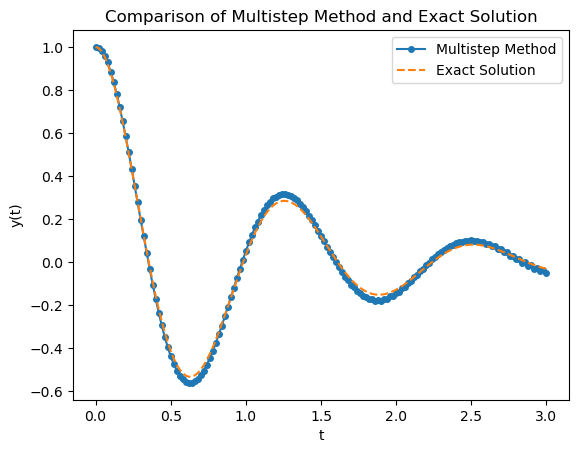
\includegraphics[width=0.4\textwidth]{Q3c1.png}
            \caption{Plot of exact solution and numerical solution using multi-step method from part (a)}
            %\label{fig:my_label}
        \end{figure}
        \begin{figure}[H]
            \centering
            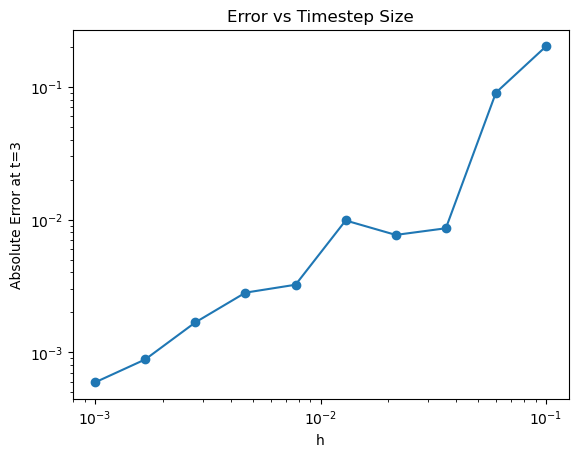
\includegraphics[width=0.4\textwidth]{Q3c2.png}
            \caption{Log-Log plot of absolute error between numerical and exact values of $y$ at $t = 3$ as a function of $h$}
            %\label{fig:my_label}
        \end{figure}

        \item Look at \texttt{Homework2.ipynb} for the solution. Below is a log-log plot of the absolute error of $y$ at $t=3$ as a function of $h$ when using forward Euler steps to set $\vec{y}_1$ and $\vec{y}_2$. 
        \begin{figure}[H]
            \centering
            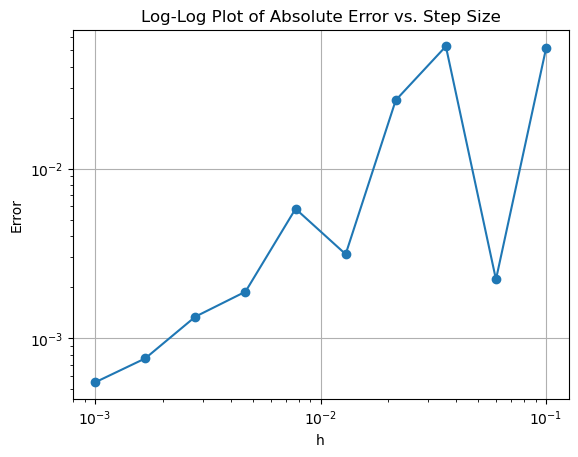
\includegraphics[width=0.4\textwidth]{Q3d.png}
            \caption{Log-Log plot of absolute error of $y$ at $t=3$ as a function of $h$ when using forward Euler steps to set $\vec{y}_1$ and $\vec{y}_2$}
            %\label{fig:my_label}
        \end{figure}
        From the plot we can see that the order of accuracy is $1$ as the slope was $\approx 0.8$. This is because the forward Euler method is a first-order method. So then when we use it to set $\vec{y}_1$ and $\vec{y}_2$, we are limiting the overall accuracy of the multi-step method to first-order.
\end{enumerate}




\begin{problem} \\ 
    \textbf{Linear Difference Equation:} \\
    \begin{enumerate}[(a)]
        \item Find the general solution of the linear difference equation 
        \[U_{n+3} + 2U_{n+2} - 4U_{n+1} - 8U_n =0. \quad \quad \quad \text{(3)} \]
        \item Determine the particular solution with initial data $U_0=4$, $U_1=-2$, and $U_2=8$.
        \item Consider the iteration \[
            \left(\begin{array}{c} U_{n+1} \\ U_{n+2} \\ U_{n+3} \end{array} \right)
            =
            \left( \begin{array}{ccc} 0 & 1 & 0 \\ 0 & 0 & 1 \\ 8 & 4 & -2 \end{array} \right)
            \left(\begin{array}{c} U_{n} \\ U_{n+1} \\ U_{n+2} \end{array} \right),
            \] 
            which we can define as $\mathbf{U}_{n+1} = A \mathbf{U}_n$. The matrix $A$ is called the companion matrix for the difference equation in (3). A general solution of the difference equation is given by $\mathbf{U}_{n} = A^n \mathbf{U}_0$. If $A=RJR^{-1}$ is the Jordan canonical form for $A$, then $A^n = RJ^n R^{-1}$. Determine the eigenvalues and Jordan canonical form for this matrix and show how this is related to the general solution found in part (a).
    \end{enumerate}
\end{problem}



\begin{enumerate}[(a)]
    \item We want to find the general solution of the linear difference equation:
        $$U_{n+3} + 2U_{n+2} - 4U_{n+1} - 8U_n = 0$$

        For a linear homogeneous difference equation, we assume a solution of the form $U_n = r^n$ and substitute:

        $$r^{n+3} + 2r^{n+2} - 4r^{n+1} - 8r^n = 0$$
        $$\iff r^n(r^3 + 2r^2 - 4r - 8) = 0$$

        From this we get the characteristic equation $r^3 + 2r^2 - 4r - 8 = 0$. Factoring this equation gives: 
        \begin{align*}
            r^3 + 2r^2 - 4r - 8 &= r^2(r + 2) - 4(r + 2) \\
            &= (r^2 - 4)(r + 2) \\
            &= (r - 2)(r + 2)^2 = 0
        \end{align*}

        Thus we have that the roots are $r_1 = 2$ and $r_2 = -2$ with multiplicity $2$. From this we can find the general solution where for $r_1 = 2$ we get $C_1 \cdot 2^n$ and $r_2 = -2$ the contribution is $C_2 \cdot (-2)^n + C_3 \cdot n \cdot (-2)^n$.
        Thus we have that the general solution is:

        \begin{align*}
            U_n &= C_1 2^n + C_2 (-2)^n + C_3 n (-2)^n \\
            &= C_1 2^n + (C_2 + C_3 n) (-2)^n
        \end{align*}

        \item From part (a), we have that the general solution is:
            \[ U_n = C_1 2^n + C_2 (-2)^n + C_3 n (-2)^n \]

            Then, utilizing the initial conditions we have that for $n = 0$: $U_0 = 4$
            \begin{align*}
                U_0 &= C_1 \cdot 2^0 + C_2 \cdot (-2)^0 + C_3 \cdot 0 \cdot (-2)^0 \\
                4 &= C_1 \cdot 1 + C_2 \cdot 1 + C_3 \cdot 0 \\
                4 &= C_1 + C_2 \tag{Q4.1}
            \end{align*}

            For $n = 1$: $U_1 = -2$
            \begin{align*}
                U_1 &= C_1 \cdot 2^1 + C_2 \cdot (-2)^1 + C_3 \cdot 1 \cdot (-2)^1 \\
                -2 &= C_1 \cdot 2 + C_2 \cdot (-2) + C_3 \cdot 1 \cdot (-2) \\
                -2 &= 2C_1 - 2C_2 - 2C_3 \tag{Q4.2}
            \end{align*}
            
            For $n = 2$: $U_2 = 8$

            \begin{align*}
                U_2 &= C_1 \cdot 2^2 + C_2 \cdot (-2)^2 + C_3 \cdot 2 \cdot (-2)^2 \\
                8 &= C_1 \cdot 4 + C_2 \cdot 4 + C_3 \cdot 2 \cdot 4 \\
                8 &= 4C_1 + 4C_2 + 8C_3 \tag{Q4.3}
            \end{align*}
           

            Thus, from (Q4.1), (Q4.2), and (Q4.3) get the following system of equations.
            1. $C_1 + C_2 = 4$
            2. $2C_1 - 2C_2 - 2C_3 = -2 \iff C_1 - C_2 - C_3 = -1$
            3. $4C_1 + 4C_2 + 8C_3 = 8 \iff C_1 + C_2 + 2C_3 = 2$

            Putting this into an extended matrix we have:
            $$ \begin{pmatrix}
            1 & 1 & 0 & 4 \\
            1 & -1 & -1 & -1 \\
            1& 1& 2& 2 \\
            \end{pmatrix} \xrightarrow{\text{RREF}}
            \begin{pmatrix}
            1 & 0 & 0 & 1 \\
            0 & 1 & 0 & 3 \\
            0 & 0 & 1 & -1 \\
            \end{pmatrix} $$

            So then $C_1 = 1$, $C_2 = 3$, and $C_3 = -1$. Next we have that the particular solution is given by:

            \begin{align*}
                U_n &= 1 \cdot 2^n + 3 \cdot (-2)^n + (-1) \cdot n \cdot (-2)^n \\
                &= 2^n + 3(-2)^n - n(-2)^n \\
                &= 2^n + (3 - n)(-2)^n \tag{Q4(b) Ans}
            \end{align*}

            To verify we can see that
            \begin{itemize}
                \item $U_0 = 2^0 + (3 - 0)(-2)^0 = 1 + 3(1) = 4$
                \item $U_1 = 2^1 + (3 - 1)(-2)^1 = 2 + 2(-2) = 2 - 4 = -2$
                \item $U_2 = 2^2 + (3 - 2)(-2)^2 = 4 + 1(4) = 4 + 4 = 8$
            \end{itemize}
            \item To find the eigenvalues and Jordan canonical form of the companion matrix 
            \[
            A = \begin{pmatrix}
            0 & 1 & 0 \\
            0 & 0 & 1 \\
            8 & 4 & -2
            \end{pmatrix},
            \]
            we first compute the characteristic polynomial of $A$. The characteristic equation is given by $\det(A - \lambda I) = 0$, where $I$ is the identity matrix. Subtracting $\lambda I$ from $A$, we have:
            \[
            A - \lambda I = \begin{pmatrix}
            -\lambda & 1 & 0 \\
            0 & -\lambda & 1 \\
            8 & 4 & -2 - \lambda
            \end{pmatrix}.
            \]

            The determinant is:
            \[
            \det(A - \lambda I) = \begin{vmatrix}
            -\lambda & 1 & 0 \\
            0 & -\lambda & 1 \\
            8 & 4 & -2 - \lambda
            \end{vmatrix}.
            \]

            Expanding along the first row:
            \begin{align*}
                \det(A - \lambda I) &= (-\lambda) \begin{vmatrix}
                -\lambda & 1 \\
                4 & -2 - \lambda
                \end{vmatrix} - 1 \begin{vmatrix}
                0 & 1 \\
                8 & -2 - \lambda
                \end{vmatrix} \\
                &= (-\lambda)(\lambda^2 + 2\lambda - 4) - 1(-8) \\
                &= -\lambda^3 - 2\lambda^2 + 4\lambda + 8 \\
                &= -(\lambda^3 + 2\lambda^2 - 4\lambda - 8).
            \end{align*}

            From part (a), we already factored the characteristic polynomial:
            \[
            \lambda^3 + 2\lambda^2 - 4\lambda - 8 = (\lambda - 2)(\lambda + 2)^2.
            \]

            Thus, the eigenvalues are $\lambda_1 = 2$ (with multiplicity 1) and $\lambda_2 = -2$ (with multiplicity 2).

            The Jordan form of $A$ is:
            \[
            J = \begin{pmatrix}
            2 & 0 & 0 \\
            0 & -2 & 1 \\
            0 & 0 & -2
            \end{pmatrix}.
            \]

            The eigenvector corresponding to $\lambda_1 = 2$ is found by solving $(A - 2I)\vec{v} = 0$. Similarly, for $\lambda_2 = -2$, we solve $(A + 2I)\vec{v} = 0$ and find the generalized eigenvector.

            The general solution of the difference equation is related to the Jordan form as:
            \[
            \mathbf{U}_n = A^n \mathbf{U}_0 = RJ^n R^{-1} \mathbf{U}_0,
            \]
            where $R$ is the matrix of eigenvectors and generalized eigenvectors.

            This confirms that the general solution derived in part (a) matches the structure of the solution obtained using the Jordan canonical form.
\end{enumerate}





\newpage 
\section*{References}
\begin{enumerate}
    \item \url{https://www.math.kent.edu/~reichel/publications/toep3.pdf}
\end{enumerate}





\end{document}